\documentclass[12pt, a4paper, simple]{eskdtext}

\usepackage{env}
\usepackage{hyperref}
\usepackage{_sty/gpi_lst}
\usepackage{_sty/gpi_toc}
\usepackage{_sty/gpi_p}
\usepackage{_sty/gpi_t}

% Код
\def \gpiDocTypeNum {81}
\def \gpiDocVer {02}
\def \gpiCode {\gpiLetterI\gpieLetterII\gpiLetterIII.\gpiStudentGroupName\gpiStudentGroupNum.\gpiStudentCard-0\gpiDocNum~\gpiDocTypeNum~\gpiDocVer}

\def \gpiDocTopic {\gpiFIObig\/Q}

% Графа 1 (наименование изделия/документа)
\ESKDcolumnI {\ESKDfontIII \gpiTopic \\ \gpiDocTopic}

% Графа 2 (обозначение документа)
\ESKDsignature {\gpiCode}

% Графа 4 (литералы)
\ESKDcolumnIVfI {\gpiLetterI}
\ESKDcolumnIVfII {\gpieLetterII}
\ESKDcolumnIVfIII {\gpiLetterIII}

% Графа 9 (наименование или различительный индекс предприятия) задает команда
\ESKDcolumnIX {\gpiDepartment}

% Графа 11 (фамилии лиц, подписывающих документ) задают команды
\ESKDcolumnXIfI {\gpiStudentSurname}
\ESKDcolumnXIfII {\gpiTeacherSurname}
\ESKDcolumnXIfV {\gpiTeacherSurname}

\begin{document}
    \begin{ESKDtitlePage}
        \hspace{0pt}\\
        \vfill
        \begin{center}
            \textbf{\ESKDfontV \gpiTopic \\ \gpiDocTopic}
        \end{center}
        \vfill
        \hspace{0pt}\\
    \end{ESKDtitlePage}
    
    \tableofcontents                                
    \thispagestyle{empty} % удаляет нумерацию страниц, которую создает библиотека
    \newpage

    \section{Краткое функциональное описание системы}

Система обеспечивает первичный ввод типизированных документов бухгалтерского учета
(операция, сумма, базовые аналитика по операции).
С последующей разноской (контировкой) данного документа в регистрационный журнал (РЖ). 

Далее из РЖ формируется книга счетов (КС),
которая служит основанием для формирования балансовой отчетности (БО).

Данная система обеспечивает минимальный комплект БО:
\begin{itemize}
    \item оборотно-сальдовая ведомость;
    \item балансовая ведомость (заглушка);
    \item журнал-ордер (заглушка).
\end{itemize}

При формировании первичных документов используются картотеки справочного характера (справочники):
\begin{itemize}
    \item Типовые хозяйственные операции (ТХО);
    \item Настройка APMa.
\end{itemize}

Архивирование системы обусловлено:
\begin{itemize}
    \item Копированием системы (заглушка);
    \item Восстановлением системы (заглушка);
\end{itemize}

\newpage

    \section{Материалы предварительного проектирования системы}
\subsection{Функциональная схема обработки данных}

\begin{figure}[!htb]
    \centering
    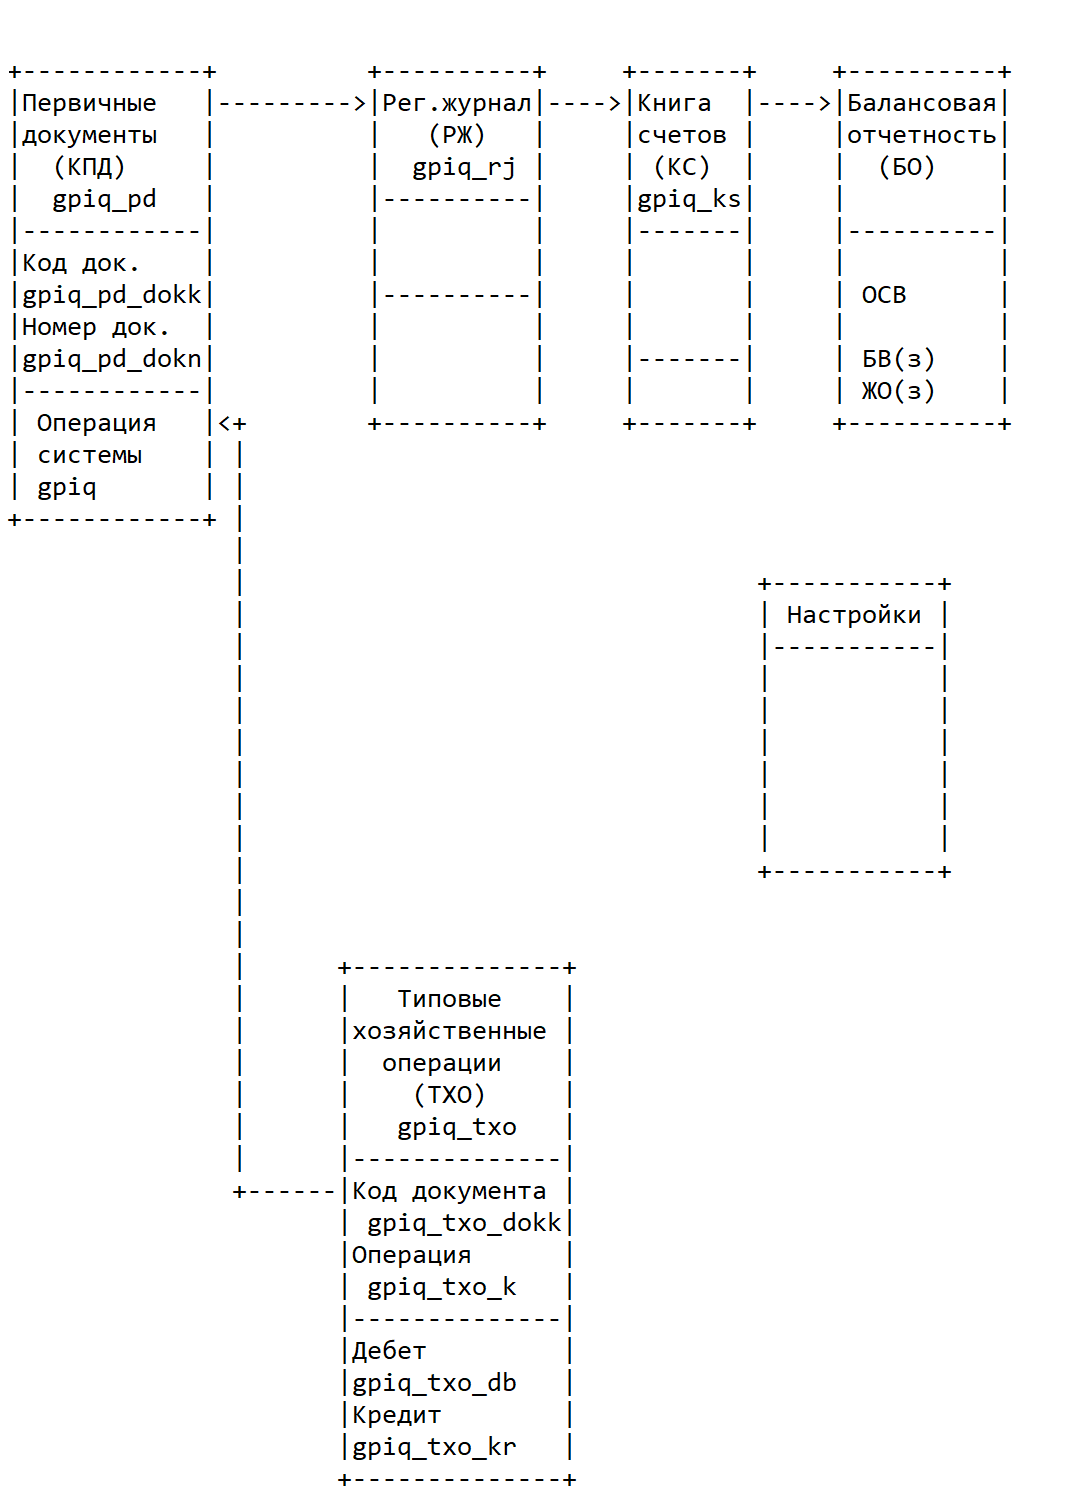
\includegraphics[height=16cm]
        {_assets/gpiq_part2.png}
    \caption{Функциональная схема обработки данных}
    \label{fig:gpiq_part2}
\end{figure}

\subsection{Описание картотек}

Картотеки:

\begin{itemize}
    \item Первичные документы gpiq\_ps\_s;
    \item[] \hspace{0pt}
    \item Регистрационный журнал (РЖ) gpiq\_rj\_s;
    \item Книга счетов (КС) gpiq\_ks;
    \item[] \hspace{0pt}  
    \item Типовые хозяйственные операции (ТХО) gpiq\_txo\_s;
    \item[] \hspace{0pt}     
    \item Настройки системы gpiq\_nst\_s:
    \item Настройки интервалов счетов;
    \item Настройки текущей даты.
\end{itemize}

\begin{table}[h!p]
    \centering
    \scriptsize
    \caption{Первичные документы gpiq\_pd}
    \begin{tabular}{|l|l|l|} 

\hline
\textbf{Реквизит}                   &\textbf{Обозначение}   &\textbf{Тип и значность}   \\ \hline
код документа                       &gpiq\_pd\_dokk         &varchar(4)                 \\ \hline
номер документа                     &gpiq\_pd\_dokn         &int                        \\ \hline
дата документа                      &gpiq\_pd\_dokd         &date                       \\ \hline
операции                            &gpiq\_pd\_to           &varchar(10)                \\ \hline
дебет счет *txo                     &gpiq\_pd\_db           &int                        \\ \hline
дебет счет субсчет наименование *txo&gpiq\_pd\_dbn          &varchar(10)                \\ \hline
кредит  *txo                        &gpiq\_pd\_kr           &int                        \\ \hline
кредит название*txo                 &gpiq\_pd\_krn          &varchar(10)                \\ \hline
сумма                               &gpiq\_pd\_rub          &int                        \\ \hline

    \end{tabular}
\end{table}

% \begin{table}[h!p]
%     \centering
%     \scriptsize
%     \caption{Виды аналитики gpia\_va}
%     \begin{tabular}{|l|l|l|} 

%                                                                                \hline
% \textbf{Реквизит}       &\textbf{Обозначение}   &\textbf{Тип и значность}   \\ \hline
% поле связи  	  =0    &gpia\_va\_0            &c1                         \\ \hline
% вид аналитики           &gpia\_va\_k            &c3                         \\ \hline
% название вида аналитики &gpia\_va\_n            &c15                        \\ \hline

%     \end{tabular}
% \end{table}

\begin{table}[h!p]
    \centering
    \scriptsize
    \caption{Регистрационный журнал (РЖ) gpiq\_rj}
    \begin{tabular}{|l|l|l|} 

                                                                                       \hline
\textbf{Реквизит}               &\textbf{Обозначение}   &\textbf{Тип и значность}   \\ \hline
дата операции                   &gpiq\_rj\_data         &date                       \\ \hline
код оправдательного документа   &gpiq\_rj\_dokk         &varchar(7)                 \\ \hline
номер документа                 &gpiq\_rj\_dokn         &int                        \\ \hline
дата документа                  &gpiq\_rj\_dokd         &date                       \\ \hline
содержание операции             &gpiq\_rj\_to           &varchar(50)                \\ \hline
дебет, счет                     &gpiq\_rj\_db           &int                        \\ \hline
дебет, название                 &gpiq\_rj\_dbn          &varchar(10)                \\ \hline
кредит, счет                    &gpiq\_rj\_kr           &int                        \\ \hline
кредит название                 &gpiq\_rj\_krn          &varchar(10)                \\ \hline
Сумма                           &gpiq\_rj\_rub          &int                        \\ \hline

    \end{tabular}
\end{table}

\begin{table}[h!p]
    \centering
    \scriptsize
    \caption{Книга счетов(КС) gpiq\_ks}
    \begin{tabular}{|l|l|l|} 

                                                                                   \hline
\textbf{Реквизит}               &\textbf{Обозначение}   &\textbf{Тип и значность}   \\ \hline
дата операции                   &gpiq\_ks\_data         &date                       \\ \hline
код оправдательного документа   &gpiq\_ks\_dokk         &varchar(4)                 \\ \hline
номер документа                 &gpiq\_ks\_dokn         &int                        \\ \hline
дата документа                  &gpiq\_ks\_dokd         &date                       \\ \hline
операции                        &gpiq\_ks\_to           &varchar(50)                \\ \hline
счет                            &gpiq\_ks\_s            &int                        \\ \hline
счёт название                   &gpiq\_ks\_sn           &varchar(10)                \\ \hline
кор. счёт                       &gpiq\_ks\_ks           &int                        \\ \hline
кор. счет наименование          &gpiq\_ks\_ksn          &varchar(10)                \\ \hline
сумма дб                        &gpiq\_ks\_rubdb        &int                        \\ \hline
сумма кр                        &gpiq\_ks\_rubkr        &int                        \\ \hline

    \end{tabular}
\end{table}

% \begin{table}[h!p]
%     \centering
%     \scriptsize
%     \caption{Определение первичных документов gpia\_opd}
%     \begin{tabular}{|l|l|l|} 

%                                                                                    \hline
% \textbf{Реквизит}           &\textbf{Обозначение}   &\textbf{Тип и значность}   \\ \hline
% поле связи       =0         &gpia\_opd\_0           &c1                         \\ \hline
% код документа               &gpia\_opd\_k           &c3                         \\ \hline
% наименование документа      &gpia\_opd\_n           &c10                        \\ \hline
% вид аналитики 1  < ---  va  &gpia\_opd\_av1         &c3                         \\ \hline
% тип аналитики 1    =д, к, x &gpia\_opd\_avt1        &c1                         \\ \hline
% виды аналитики 2            &gpia\_opd\_av2         &c3                         \\ \hline
% тип аналитики 2             &gpia\_opd\_avt2        &c1                         \\ \hline
% вид аналитики 3             &gpia\_opd\_av3         &c3                         \\ \hline
% тип аналитики 2             &gpia\_opd\_avt3        &c1                         \\ \hline

%     \end{tabular}
% \end{table}

\begin{table}[h!p]
    \centering
    \scriptsize
    \caption{Типовые хозяйственные операции(ТХО) gpiq\_txo}
    \begin{tabular}{|l|l|l|} 

                                                                                           \hline
\textbf{Реквизит}                   &\textbf{Обозначение}   &\textbf{Тип и значность}   \\ \hline
код документа                       &gpiq\_txo\_dokk        &varchar(4)                 \\ \hline
операции                            &gpiq\_txo\_k           &varchar(10)                \\ \hline
дебет, счёт                         &gpiq\_txo\_db          &int                        \\ \hline
дебет, название                     &gpiq\_txo\_dbn         &varchar(10)                \\ \hline
кредит                              &gpiq\_txo\_kr          &int                        \\ \hline
кредит, название                    &gpiq\_txo\_krn         &varchar(10)                \\ \hline

    \end{tabular}
\end{table}

% \begin{table}[h!p]
%     \centering
%     \scriptsize
%     \caption{План счетов(ПС) gpia\_ps}
%     \begin{tabular}{|l|l|l|} 

%                                                                                            \hline
% \textbf{Реквизит}                   &\textbf{Обозначение}   &\textbf{Тип и значность}   \\ \hline
% поле связи        =0                &gpia\_ps\_0            &c1                         \\ \hline
% счет                                &gpia\_ps\_s            &n2                         \\ \hline
% название счета                      &gpia\_ps\_n            &c10                        \\ \hline
% тип счета          = а, п, x        &gpia\_ps\_typ          &c1                         \\ \hline
% вид аналитики 1 из VA               &gpia\_ps\_av1          &c3                         \\ \hline
% вид аналитики 2 из VA               &gpia\_ps\_av2          &c3                         \\ \hline

%     \end{tabular}
% \end{table}

% \begin{table}[h!p]
%     \centering
%     \scriptsize
%     \caption{Коды аналитического учёта(КАУ) gpia\_kau}
%     \begin{tabular}{|l|l|l|} 

%                                                                                \hline
% \textbf{Реквизит}       &\textbf{Обозначение}   &\textbf{Тип и значность}   \\ \hline
% поле связи          =0  &gpia\_kau\_0           &c1                         \\ \hline
% вид аналитики           &gpia\_kau\_k           &c5                         \\ \hline
% вид аналитики           &gpia\_kau\_n           &c15                        \\ \hline

%     \end{tabular}
% \end{table}

\begin{table}[h!p]
    \centering
    \scriptsize
    \caption{Настройки системы gpiq\_nst}
    \begin{tabular}{|l|l|l|} 

                                                                               \hline
\textbf{Реквизит}       &\textbf{Обозначение}   &\textbf{Тип и значность}   \\ \hline
дата текущая            &gpiq\_nst\_datat       &date                       \\ \hline
интервал с              &gpiq\_nst\_datas       &date                       \\ \hline
интервал до             &gpiq\_nst\_datado      &date                       \\ \hline
cчёт                    &gpiq\_nst\_s           &int                        \\ \hline
название счёта          &gpiq\_nst\_sn          &varchar(10)                \\ \hline
название фирмы          &gpiq\_nst\_firma       &varchar(10)                \\ \hline

    \end{tabular}
\end{table}

\subsection{Описание работ}

\begin{table}[h!p]
    \centering
    \scriptsize
    \caption{Описание работ}
    \begin{tabular}{|p{8cm}|p{8cm}|} 

% = = = = = = = = = =

\hline

% = = = = = = = = = =

\textbf{Группа работ}
&
\textbf{Работы}
\\ \hline

% = = = = = = = = = =

Формирование и разноска первичных документов \par
\hspace{0pt} \par
\textbf{gpiq\_Документы}
&
- gpiq\_Ввод текущей даты \par
- gpiq\_Ввод и разноска первичных документов (ПД)
\\ \hline

% = = = = = = = = = =

Работа с регистрационным журналом \par
\hspace{0pt} \par
\textbf{gpiq\_РЖ}
&
- gpiq\_Просмотр РЖ \par
- gpiq\_Формирование книги счетов из рег. журнала \par
- gpiq\_Просмотр КС
\\ \hline

% = = = = = = = = = =

Формирование балансовой отчетности \par
\hspace{0pt} \par
\textbf{gpiq\_БО}
&
- gpiq\_Опеделение отчетных форм \par
- gpiq\_Оборотно-сальдовая ведомость  \par
- gpiq\_Балансовая ведомость (заглушка) \par
- gpiq\_Журнал-ордер (заглушка)
\\ \hline

% = = = = = = = = = =

Сопровождение картотек-справочников \par
\hspace{0pt} \par
\textbf{gpiq\_Картотеки}
&
- gpiq\_Типовые хозяйственные операции (ТХО) \par
- gpiq\_Настройка АРМа
\\ \hline

% = = = = = = = = = =

Ведение архивов \par
\hspace{0pt} \par
\textbf{gpiq\_Архивы}
&
- gpiq\_Копирование системы (заглушка) \par
- gpiq\_Восстановление системы (заглушка) \par
\\ \hline

% = = = = = = = = = =

Выход из системы \par
\hspace{0pt} \par
\textbf{gpiq\_Выход}
&
- gpiq\_Выход из системы
\\ \hline

% = = = = = = = = = =

    \end{tabular}
\end{table}

\newpage

    \section{Эксплуатационное описание системы}

\subsection{Функциональная схема обработки данных с использованием инструментальной среды}
\subsection{Описание картотек с использованием инструментальной среды}
\subsection{Скриншоты меню}
\subsection{Скриншоты картотек}
\subsection{Образцы первичных документов}
\subsection{Образцы печатных форм}

% \newpage

    \section{Электронная версия разработанной системы}

\newpage

\end{document}
